\documentclass[11pt]{scrartcl}
\usepackage[sexy]{evan}
\usepackage{graphicx}

\usepackage{answers}
\usepackage{listings}
\usepackage{xcolor}
\Newassociation{hint}{hintitem}{all-hints}
\renewcommand{\solutionextension}{out}
\renewenvironment{hintitem}[1]{\item[\bfseries #1.]}{}
\declaretheorem[style=thmbluebox,name={Theorem}]{thm}

\lstset{
    frame=tb, % draw a frame at the top and bottom of the code block
    tabsize=4, % tab space width
    showstringspaces=false, % don't mark spaces in strings
    numbers=left, % display line numbers on the left
    commentstyle=\color{green}, % comment color
    keywordstyle=\color{blue}, % keyword color
    stringstyle=\color{red} % string color
}

\begin{document}
\title{CS 170}
\author{Vishal Raman}
\thispagestyle{empty}
$ $
\vfill
\begin{center}

\centerline{\huge \textbf{CS 170 Lecture Notes, Fall 2020}}
\centerline{\Large \textbf{Algorithms and Intractable Problems} } 
\centerline{Professors: Avishay Tal, Umesh Vazirani}
\centerline{Scribe: Vishal Raman}
\end{center}
\vfill
$ $
\newpage
\thispagestyle{empty}
\tableofcontents
\newpage
%\maketitle
\section{September 1st, 2020}
\subsection{Naive Multiplication} 
Recall the example of Fibonacci: we went from a complexity of $O(2^n) \rightarrow O(n^2) \rightarrow O(f(n))$, where $f(n)$ is the runtime for multiplying $n$-bit numbers.  The naive algorithm is the usual multiplication algorithm for multiplying by hand.
\begin{center}
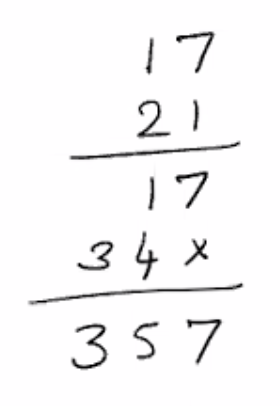
\includegraphics[scale=0.5]{multiply.png}
\end{center}
\begin{lstlisting}[language=python, caption={Naive n-bit multiplication}]
function multiply(x, y):
Input: n-bit integers, x, y, y >= 0
Output: Product

    if (y == 0) return 0;
    s = multiply(x, floor(y/2))
    if y is even:
    	return 2z
    else
    	return x+2z
\end{lstlisting}
If we write $x = \sum_{i=0}^{n-1} x_{j}2^i, y = \sum_{i=0}^{n-1} y_i 2^i$, so 
$$xy = \left (\sum_{i=0}^{n-1} x_{j}2^i\right )\left (\sum_{i=0}^{n-1} y_i 2^i\right ) = \sum_{j, k = 0}^n x_jy_k 2^{j+k}.$$
\subsection{Divide and Conquer: Karatsuba's Algorithm}
For a Divide and Conquer problem, we do the following:
\begin{enumerate}
\item  Break problem into pieces.
\item Solve pieces recursively.
\item Glue solutions of pieces to get solution of original problem.
\end{enumerate}
We first have $x$ an n-bit number that we break up into $x_L, x_R$, each $n/2$ bit numbers.  Similarly, we break $y$ into $y_L, y_R$.
\begin{center}
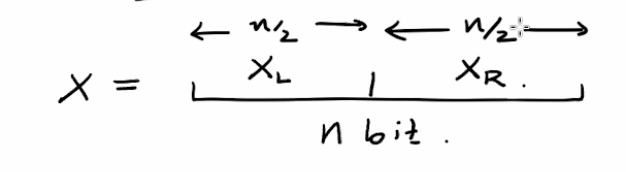
\includegraphics[scale=0.5]{dac.png}
\end{center}
Note that $x = 2^{n/2}x_L + x_R, y = 2^{n/2}y_L + y_R,$, so
$$xy = 2^n x_Lx_L + 2^{n/2}(x_Ly_R + x_Ry+L) + x_Ry_R.$$
We now have 4 multiplications, involving $n/2$-bit numbers.  Multiplication by $2^m$ can be shifting ($O(m)$ time), and addition is $O(1)$.  Hence, we have a recurrence equation for the runtime,
$$T(n) = 4T\left (\frac{n}{2}\right ) + O(n).$$
\begin{center}
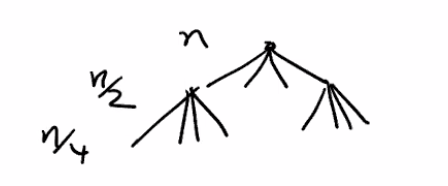
\includegraphics[scale=0.5]{rec.png}
\end{center}
Note that the depth of the recursion tree is $\log n$ and there are $4^{\log n} = n^2$ leaves.  But this would have the same runtime as the naive algorithm, so more work is required to optimize.
\end{document}
